\section{Equalizing}
Equalizing effect is done with a bank of bandpass filters using third-octave parametric from \SI{20}{\hertz} to \SI{20}{\kilo\hertz} which are divided by a fixed or customized frequency distance. The analog equalizer often has a fixed distance while the digital equalizer is more flexible and often has customized frequency distance. This bandpass filter is able to either amplify or attenuate the gain of the specified frequency. The \autoref{fig:analog_equalizer} shows an analog equalizer with traditional third-octave parametric. \cite{nordic}
\todo[inline]{Jonas: Fix your citep and explain third-octave}

\begin{figure} [htbp]
 \centering
  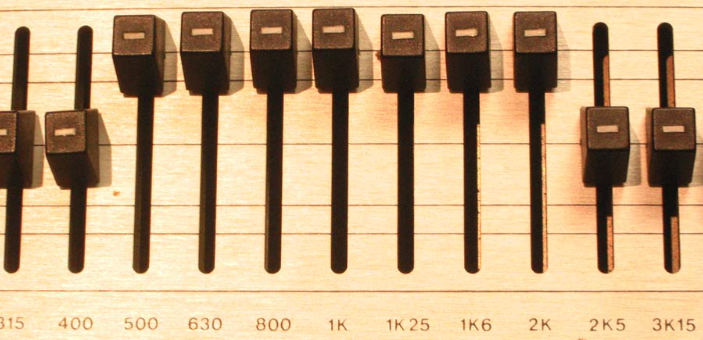
\includegraphics[width=0.8\textwidth]{analog_equalizer}
  \caption{The photo shows an example of an analog equalizer}
  \label{fig:analog_equalizer}
\end{figure}

\todo[inline]{Mohamed : Maybe add why they will affect each other}
One amplified bandpass filter will interfere with the other neighboring filters, thus the frequency response will be different than what can be expected with ideal filters on the analog equalizer output. The following \autoref{fig:analog_equalizer_respond} shows the analog frequency response of the above analog equalizer \autoref{fig:analog_equalizer}.

\begin{figure} [htbp]
 \centering
  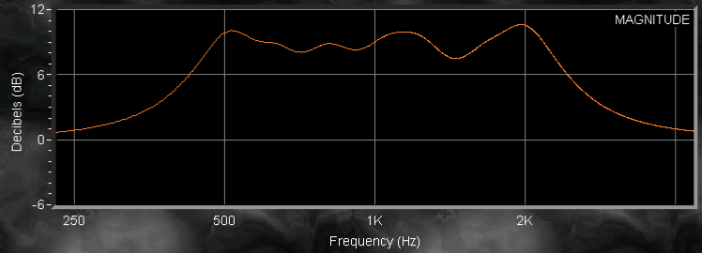
\includegraphics[width=0.8\textwidth]{analog_equalizer_respond}
  \caption{The photo shows the response of the equalizer at \autoref{fig:analog_equalizer} }
  \label{fig:analog_equalizer_respond}
\end{figure}

The interference effects on the side lying bandpass filter can easily be avoided by using an digital equalizer with third-octave raised cosine characteristics. The difference between the  bandpass filter characteristics and the one with a raised-cosine are shown in \autoref{fig:raised_cosine_vs_traditional}

\begin{figure} [htbp]
 \centering
  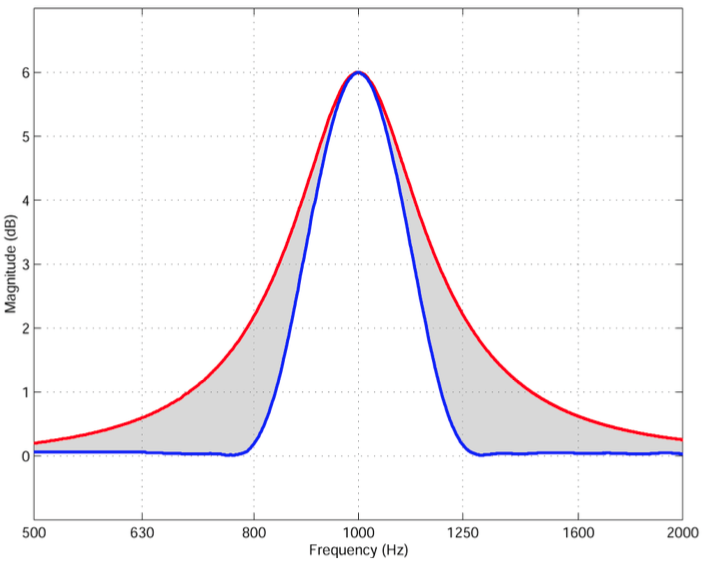
\includegraphics[width=0.7\textwidth]{raised_cosine_vs_traditional}
  \caption{The photo shows the raised cosine bandpass filter characteristics versus traditional characteristics of third-octave bandpass filter %\citep{nordic}
  }
  \label{fig:raised_cosine_vs_traditional}
\end{figure}



When using third-octave raised cosine bandpass filter, it is possible to make an equalizer where neighboring filters do not interfere with each other, because a raised cosine filter does not leak into other third-octave bands like the traditional filter does. With this kind of filter it is possible to make a perfectly flat frequency response, and it is very close to an ideal equalizer. The \autoref{fig:raised_cosine_respond} shows the frequency response of a third-octave raised cosine equalizer designed by Dolby lake with the same gain and frequency settings as the analog equalizer at \autoref{fig:analog_equalizer}.

\begin{figure} [htbp]
 \centering
  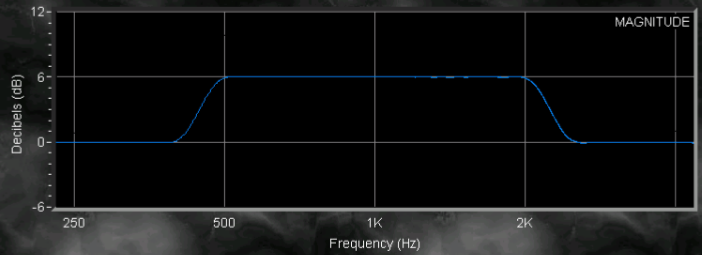
\includegraphics[width=0.8\textwidth]{raised_cosine_respond}
  \caption{The photo shows an third-octave raised cosine equalizer frequency response  %\citep{nordic}
  }
  \label{fig:raised_cosine_respond}
\end{figure}


The equalizer is used to compensate for the changes in sound due to different room characteristics, because the sound can be completely different in different rooms. The room characteristics will or can amplify or attenuate some frequency, and therefore the equalizer is very important to adjust the frequency in every new room. 



http://www.howtogeek.com/59467/htg-explains-what-is-an-equalizer-and-how-does-it-work/

http://www.nordicsales.dk/imgdb/docs/lakewh_981.pdf
